\chapter{Project Initialization}
\section{Feasibility}
\label{sec-feasibility}
\begin{itemize}
\item We wish to create a system, which having been trained from sentences annotated with emotions portrayed, is capable of predicting the emotion for a new sentence.
\item We will be closely following the paper Taner Danisman and Adil Alpkocak titled \href{http://people.cs.deu.edu.tr/alpkocak/Papers/AISB08.pdf}{\textbf{Feeler: Emotion Classification of Text Using Vector Space Model}}.
\item We will need to build a lexicon, which is basically an ordered set of all \emph{good} words in the training data.
\item For each sentence we will build a weight vector of all terms in the lexicon.
\item The weights are calculated using the \textbf{tf-idf} technique.
\item For each emotion class we take the mean of all vectors within it.
\item We will be utilizing python for developing the application and be using \textbf{nltk} for text clean up, stemming etc.
\item Estimated time to develop the project would be a month.
\end{itemize}
\begin{center}
	\begin{figure}[ht!]
	\caption{Basic architecture of solution}
	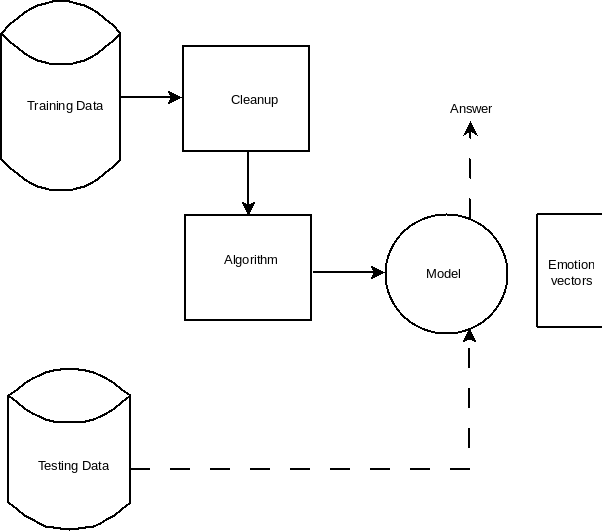
\includegraphics[scale=0.5]{ml.png}
	\end{figure}
\end{center}
\section{Dataset}
\label{sec-dataset}
\begin{itemize}
\item The paper mentions the \href{https://github.com/bogdanneacsa/tts-master/blob/master/ISEAR/DATA.csv}{ISEAR} dataset, which is composed of around 15000 annotated sentences.
\end{itemize}
\section{Scope}
\begin{itemize}
\item At its core, the idea is to find median vectors corresponding to each emotion (joy, sadness, anger, \ldots) and then find the cosine similarity of the new vector composed from test input with the former. The highest similarity vector will be the winner.
\item Other than implementing their proposed solution, we will also try to incorporate methods like bayesian classification and neural networks and analyse the results.
\item If time permits, we will build some application around our system.
\end{itemize}
